\documentclass[compress,mathserif]{beamer}
\usetheme{sthlm}

%-=-=-=-=-=-=-=-=-=-=-=-=-=-=-=-=-=-=-=-=-=-=-=-=
%        LOADING BEAMER PACKAGES
%-=-=-=-=-=-=-=-=-=-=-=-=-=-=-=-=-=-=-=-=-=-=-=-=

\usepackage{
booktabs,
datetime,
dtk-logos,
graphicx,
multicol,
pgfplots,
ragged2e,
tabularx,
tikz,
wasysym,
multirow,
float,
caption,
subcaption,
amsmath,
mathptmx,
animate
}

\usepackage[scaled=0.9]{helvet}
\usepackage{courier}

\usefonttheme[onlymath]{serif}

\definecolor{mygreen}{RGB}{113, 166, 70}
\definecolor{myblue}{RGB}{68, 140, 185}
\definecolor{myred}{RGB}{217, 98, 55}
\definecolor{mypurple}{RGB}{83, 65, 126}
\definecolor{solviaveis}{RGB}{188, 207, 241}

\pgfplotsset{compat=1.8}

\usepackage[utf8]{inputenc}
\usepackage[portuguese]{babel}
\usepackage[T1]{fontenc}
\usepackage{newpxtext,newpxmath}
\usepackage{listings}

\lstset{ %
language=[LaTeX]TeX,
basicstyle=\normalsize\ttfamily,
keywordstyle=,
numbers=left,
numberstyle=\tiny\ttfamily,
stepnumber=1,
showspaces=false,
showstringspaces=false,
showtabs=false,
breaklines=true,
frame=tb,
framerule=0.5pt,
tabsize=4,
framexleftmargin=0.5em,
framexrightmargin=0.5em,
xleftmargin=0.5em,
xrightmargin=0.5em
}



%-=-=-=-=-=-=-=-=-=-=-=-=-=-=-=-=-=-=-=-=-=-=-=-=
%        LOADING TIKZ LIBRARIES
%-=-=-=-=-=-=-=-=-=-=-=-=-=-=-=-=-=-=-=-=-=-=-=-=

\usetikzlibrary{
backgrounds,
mindmap
}

%-=-=-=-=-=-=-=-=-=-=-=-=-=-=-=-=-=-=-=-=-=-=-=-=
%        BEAMER OPTIONS
%-=-=-=-=-=-=-=-=-=-=-=-=-=-=-=-=-=-=-=-=-=-=-=-=

\setbeameroption{show notes}

%-=-=-=-=-=-=-=-=-=-=-=-=-=-=-=-=-=-=-=-=-=-=-=-=
%        BEAMER COMMANDS
%-=-=-=-=-=-=-=-=-=-=-=-=-=-=-=-=-=-=-=-=-=-=-=-=


%-=-=-=-=-=-=-=-=-=-=-=-=-=-=-=-=-=-=-=-=-=-=-=-=
%
%	PRESENTATION INFORMATION
%
%-=-=-=-=-=-=-=-=-=-=-=-=-=-=-=-=-=-=-=-=-=-=-=-=

\title{Conceitos de Otimização \\ em Redes}
\subtitle{DCE692 - Pesquisa Operacional}
%\date{\small{\jobname}}
\author{\texttt{Iago Carvalho}}
\institute{\texttt{Departamento de Ciência da Computação}}

\hypersetup{
pdfauthor = {Iago A. Carvalho},      
pdfsubject = {Pesquisa Operacional},
pdfkeywords = {},  
pdfmoddate= {D:\pdfdate},          
pdfcreator = {WriteLaTeX}
}

\begin{document}

\begin{frame}
\titlepage

\end{frame}

%% --------------------------------------------------------

\begin{frame}{Otimização em redes}

Problemas em redes são aqueles que podem ser representados como uma rede

\begin{columns}[T]
    \begin{column}{.44\textwidth}
        \begin{itemize}
            \item Conjunto de elementos
            \begin{itemize}
                \item Nós
                \item Vértices
            \end{itemize}
            \item Conexões entre os elementos
            \begin{itemize}
                \item Arcos
                \item Arestas
            \end{itemize}
        \end{itemize}
    \end{column}
    \begin{column}{.54\textwidth}
        \centering 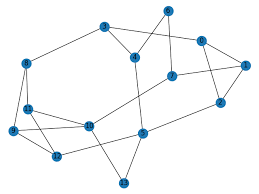
\includegraphics[width=\textwidth]{images/grafo.png}
    \end{column}
\end{columns}


\end{frame}

%% --------------------------------------------------------

\begin{frame}{Grafos}

Problemas de otimização em redes são definidos sob grafos
\begin{itemize}
    \item Uma estrutura de dados especial
    \item Representação de uma rede
    \item Talvez seja a estrutura mais útil em toda a Ciência da Computação
\end{itemize}

\vspace{1cm}

Um grafo $G$ é definido como $G = (V, E)$
\begin{itemize}
    \item $V = \{v_1, v_2, \ldots, v_n\}$ é o conjunto de vértices
    \item $E = \{e_1, e_2, \ldots, e_m\}$
    \begin{itemize}
        \item $e_i = (u, v)~|~u, v \in V$
    \end{itemize}
\end{itemize}
\end{frame}

%% --------------------------------------------------------

\begin{frame}{Direção}

Um grafo pode ser direcionado ou não-direcionado

\vspace{0.5cm}

\centering 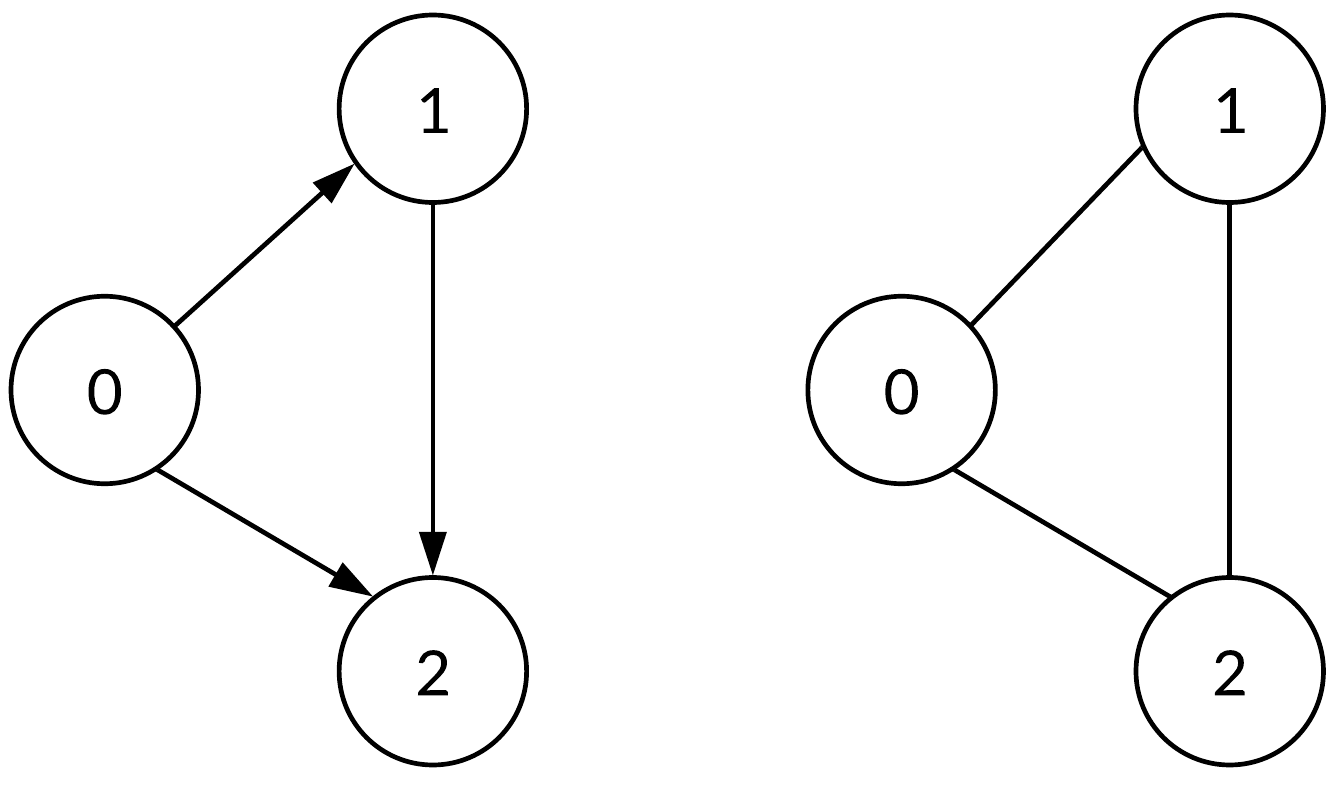
\includegraphics[width=\textwidth]{images/grafos.png}

\end{frame}

%% --------------------------------------------------------

\begin{frame}{Caminhos e ciclos}

Caminho $C = <c, e, d, c>$

\vspace{1cm}

\centering 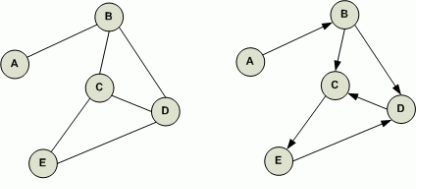
\includegraphics[width=\textwidth]{images/caminhos.png}

\end{frame}

%% --------------------------------------------------------

\begin{frame}{Adjacência e grau}

\vspace{1cm}

\centering 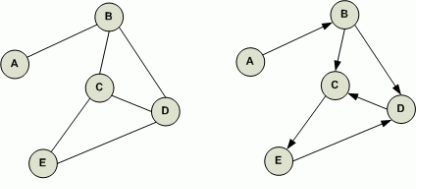
\includegraphics[width=\textwidth]{images/caminhos.png}

\end{frame}

%% --------------------------------------------------------

\begin{frame}{Fecho transitivo}

Direto e inverso

\vspace{1cm}

\centering 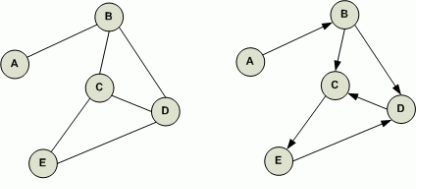
\includegraphics[width=\textwidth]{images/caminhos.png}

\end{frame}

%% --------------------------------------------------------

\begin{frame}{Fonte e sumidouro}

\vspace{1cm}

\centering 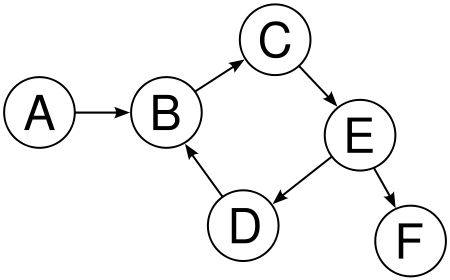
\includegraphics[width=0.9\textwidth]{images/ciclo.png}

\end{frame}

%% --------------------------------------------------------

\begin{frame}{Grafo completo}

\vspace{1cm}

\centering 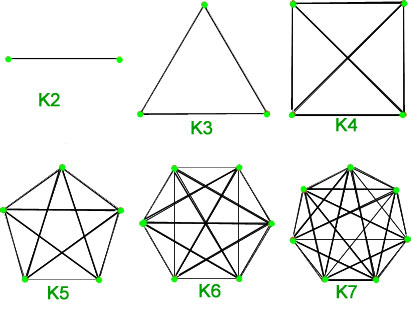
\includegraphics[width=0.9\textwidth]{images/completo.jpg}

\end{frame}

%% --------------------------------------------------------

\begin{frame}{Grafo com pesos}

\vspace{1cm}

\centering 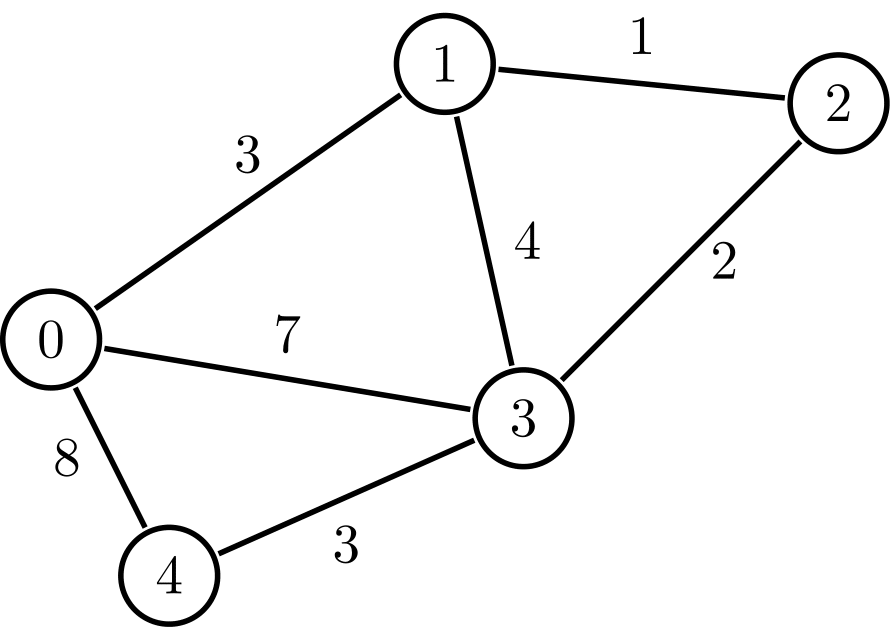
\includegraphics[width=0.9\textwidth]{images/pesos.png}

\end{frame}

%% --------------------------------------------------------

\begin{frame}{Grafo conexo}

\vspace{1cm}

\centering 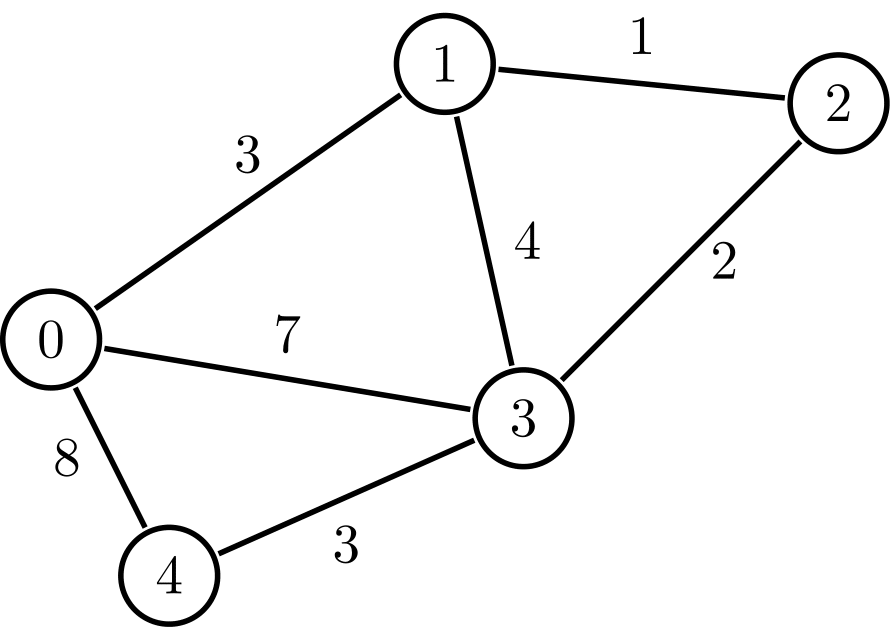
\includegraphics[width=0.9\textwidth]{images/pesos.png}

\end{frame}

%% --------------------------------------------------------

\begin{frame}{Grafo desconectado e componentes conexas}

\vspace{0.5cm}

\centering 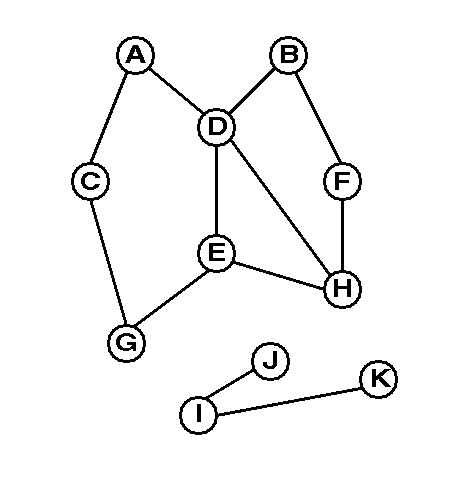
\includegraphics[width=0.75\textwidth]{images/desconectado.png}

\end{frame}

%% --------------------------------------------------------

\begin{frame}{Propriedades adicionais}

Todas estas propridades de grafos nos serão úteis para estudar problemas de otimização em redes

\vspace{0.5cm}

Grafos, por si só, são um assunto para uma disciplina inteira de graduação

\vspace{0.5cm}

Interessados em um pouco mais de propriedades de grafos podem acessar o seguinte link \href{https://www.inf.ufsc.br/grafos/definicoes/definicao.html}{\beamergotobutton{Link}}

\end{frame}

\end{document}